Diberikan graf tidak berarah $G=(V,E)$,  \textit{graph partitioning} adalah proses membagi himpunan simpul $V$ menjadi beberapa subset $V_0,V_1,\ldots V_{k-1}$ yang saling \textit{disjoint} sedemikian hinggga setiap ukuran partisi-partisi $(V_i,E_i),i\in\{0,1,\ldots, K-1\}$ kurang lebih sama dan jumlah sisi-sisi batas $E(V_i,V_j)$ yang menghubungkan partisi $V_i$ dan $V_j$ ($i\neq j$) seminimal mungkin. \cite{Schild2015} memperkenalkan algoritma Inertial Flow yang mampu membuat partisi dari graf jaringan jalan berkualitas sangat baik dengan algoritma yang sangat sederhana. Algoritma Inertial Flow diawali dengan mengurutkan simpul-simpul berdasarkan \textit{latitude} dan \textit{longitude}. Setelah simpul-simpul terurutkan, algoritma kemudian menjalankan algoritma Dinic dengan \textit{unit-capacity} \cite{Dinitz2006} menggunakan sejumlah $k$ simpul awal sebagai \textit{sources} dan sejumlah $k$ simpul terakhir sebagai \textit{sinks} dari himpunan simpul yang telah diurutkan. Proses yang terdiri dari dua langkah ini diterapkan secara rekursif pada setiap partisi yang dihasilkan hingga ukuran partisi menjadi cukup kecil (ukuran partisi kurang dari \textit{threshold} $U$ yang kita tetapkan sendiri nilainya). Dari sejumlah $k$ simpul sebagai \textit{sources} dan sejumlah $k$ simpul sebagai \textit{sinks}, dibentuk sebuah \textit{artificial source} $s$ yang dihubungkan ke semua simpul \textit{sources} dengan sisi berbobot $\infty$, serta sebuah \textit{artificial sink} $t$ yang dihubungkan dari semua simpul \textit{sinks} dengan sisi berbobot $\infty$. Kedua simpul \textit{artificial} menjadi input dari algoritma Dinic. \textit{Pseudocode} dari algoritma Inertial Flow ditunjukkan pada Algoritma~\ref{alg:inertial-flow}. Contoh hasil dari mempartisi graf jaringan jalan menggunakan algoritma Inertial Flow ditunjukkan pada Gambar~\ref{fig:inertial-flow}. Kompleksitas waktu dari algoritma Dinic adalah $O(N^2\cdot M)$ (\cite{Dinitz2006}),dimana $N$ adalah jumlah simpul dan $M$ adalah jumlah sisi. Kompleksitas waktu dari algoritma Inertial Flow adalah $O(N^2\cdot M)$ yang diberikan oleh relasi rekurens berikut:

\begin{align}
    T(N,M)&=N^2\cdot M \cdot C + T(N/2,M/2)+T(N/2,M/2) \notag \\
    &=N^2\cdot M \cdot C + 2T(N/2,M/2)  \notag \\
    &= N^2\cdot M \cdot C + \frac{ N^2}{2^2}\cdot M \cdot C + 2^2T(N/2^2,M/2^2)  \notag \\
    &= N^2\cdot M \cdot C + \frac{ N^2}{2^2}\cdot M   \cdot C + \frac{ N^2}{2^4}\cdot M \cdot C  + 2^3T(N/2^3,M/2^3)  \notag \\
    &= N^2\cdot M \cdot C + \frac{ N^2}{2^2}\cdot M \cdot C + \ldots + \frac{ N^2}{2^{2\cdot (k-1)}}\cdot M \cdot C  + 2^kT(N/2^k, M/2^k)  \notag \\
    & \text{(base case: $N/2^k = U, T(U,M/2^k)=1$)}  \notag \\ 
    &=\sum_{i=0}^{\log_2(N/U)-1} \frac{ N^2}{4^{i}}\cdot M \cdot C + \frac{N}{U}  \notag \\
    &\leq \sum_{i=0}^{\infty} \frac{ N^2}{4^i}\cdot M \cdot C+ \frac{N}{U}  \notag \\
    &= \frac{4}{3}\cdot N^2 \cdot M \cdot C \notag \\
    &=O(N^2\cdot M) \notag 
\end{align}


\begin{algorithm}
\caption{InertialFlow mengembalikan partisi-partisi dari graf $V_0,V_1,\ldots V_{k-1}$ (\cite{Schild2015})} 
\label{alg:inertial-flow}
\resizebox{\textwidth}{!}{%
\begin{minipage}{\textwidth}
\scriptsize
\begin{algorithmic}[1]
\setstretch{0.9}
\Procedure{InertialFlow}{$V, U$}
    \State $ partitionGraph \gets V $
    \State $Q \gets \emptyset : Queue$
    \State $Q.Enqueue(partitionGraph)$
    \State $partitions \gets \emptyset $
    \Procedure{computeDinic}{$currPartitionGraph$}
        \State $lines \gets \{ \{1,0\}, \{0,1\}, \{1,1\}, \{1,-1\}, \{-1,1\} \}$
        \For{$i = 0 \to 5$}
            \State $lines \gets lines \cup \{random(0,1), random(0,1) \}$
        \EndFor
        \State $bestpart_1 \gets \emptyset$
        \State $bestpart_2 \gets \emptyset$
        \State $bestCutEdgesCount \gets \infty$
        \For {$line \in lines$}
            \State $(sources,sinks) \gets $\Call{SortVerticesByLineProjection}{$line, currPartitionGraph$}
            \State $s,t \gets$ \Call{createArtificialSourceSink}{$sources,sinks$}
            \State $(cutEdges, part_1, part_2) \gets$ \Call{Dinic}{$s,t, currPartitionGraph$}
            \If{$cutEdges < bestCutEdgesCount$}
                \State $cutEdges \gets bestCutEdgesCount$
                \State $bestpart_1 \gets part_1$
                \State $bestpart_2 \gets part_2$
            \EndIf 
        \EndFor
        \State \textbf{return} $bestpart_1, bestpart_2$
    \EndProcedure
    \While{$Q \neq \emptyset $}
        \State $currPartitionGraph \gets Q.Dequeue()$
        \State $(part_1, part_2) \gets $\Call{computeDinic}{$currPartitionGraph$} 
        \If{$|part_1| > U$}
            \State $Q.Enqueue(part_1)$
        \Else 
            \State $partitions \gets partitions \cup \{part_1\}$
        \EndIf
        \If{$|part_2| > U$}
            \State $Q.Enqueue(part_2)$
        \Else 
            \State $partitions \gets partitions \cup \{part_2\}$
        \EndIf 
    \EndWhile
\EndProcedure

\end{algorithmic}
\end{minipage}%
}
\end{algorithm}



\begin{algorithm}
\caption{Dinic mengembalikan $(cutEdges, part_1, part_2)$ (\cite{Dinitz2006})} 
\label{alg:dinic}
\resizebox{\textwidth}{!}{%
\begin{minipage}{\textwidth}
\scriptsize
\begin{algorithmic}[1]
\setstretch{0.9}
\Procedure{Dinic}{$sources,sinks, currPartitionGraph$}
    \State $cutEdges \gets 0$
    \For{$e\in currPartitionGraph.E$}
        \State $e.capacity \gets 1 $ \Comment{\textit{unit-capacity} Dinic}
    \EndFor 
    \State $levels \gets \emptyset $
    \While{$true$}
        \If {\Call{bfsLevelGraph}{$s,t, currPartitionGraph, levels$} $=true$}
            \While{$true$}
                \State $flow \gets$ \Call{dfsAugmentPath}{$s,t, \infty, currPartitionGraph, levels$}
                \If {$flow = 0$}
                    \State \textbf{break}
                \EndIf
                \State $cutEdges \gets cutEdges + flow$
            \EndWhile 
        \Else 
            \State $part_1, part_2 \gets \emptyset$
            \For {$v \in currPartitionGraph.V$}
                \If {$levels[v] \neq \infty$}
                    \State $part_1 \gets part_1 \cup \{v\}$
                \Else 
                    \State $part_2 \gets part_2 \cup \{v\}$
                \EndIf
            \EndFor 
            \State \textbf{return} $(cutEdges, part_1, part_2)$
        \EndIf 
    \EndWhile 
\EndProcedure

\Procedure{bfsLevelGraph}{$s,t, currPartitionGraph, levels$}: $boolean$
    \For{$v\in currPartitionGraph.V$}
        \State $levels[v] \gets \infty $
    \EndFor 
    \State $Q \gets \emptyset : Queue$
    \State $Q.Enqueue(s)$
    \State $levels[s] \gets 0$
    \While {$Q \neq \emptyset$}
        \State $u \gets Q.Dequeue()$
        \State $level_u \gets levels[u]$
        \State $level \gets level_u +1 $
        \If {$u = t $}
            \State \textbf{break}
        \EndIf 
        \For {$e\in currPartitionGraph.E_u$}
            \State $v \gets e.v$
            \State $residual \gets e.capacity - e.flow$
            \If {$residual>0 \textbf{ and } levels[v] = \infty$}
                \State $levels[v]\gets level$
                \State $Q.Enqueue(v)$
            \EndIf 
        \EndFor
    \EndWhile
    \State \textbf{return} $levels[t]  \neq  \infty$
\EndProcedure

\Procedure{dfsAugmentPath}{$u, t, flow, currPartitionGraph, levels$}: $\mathbb{R}$
    \If {$u =t \textbf{ or } flow = 0$}
        \State \textbf{return} $flow$
    \EndIf 

    \While {$currPartitionGraph.lastIndex[u] < currPartitionGraph.|E_u |$}
        \State $j \gets currPartitionGraph.lastIndex[u]  $
        \State $e \gets  currPartitionGraph.E_u[j] $
        \State $v \gets e.v$
        \State $residual \gets e.capacity - e.flow$
        \If {$levels[v]  \neq  levels[u]+1$}
            \State \textbf{continue}
        \EndIf 
        \If{ \Call{dfsAugmentPath}{$v,t, \min\{residual,flow\}$} $>0$}
            \State $e.flow \gets e.flow + flow$
            \State $\overleftarrow{e} \gets currPartitionGraph.\overleftarrow{E}_u[j] $
            \State $\overleftarrow{e} \gets \overleftarrow{e} -flow$
            \State \textbf{return} $flow$
        \EndIf
        \State $currPartitionGraph.lastIndex[u]  \gets currPartitionGraph.lastIndex[u]  +1 $
    \EndWhile
    \State \textbf{return } $0.0$
\EndProcedure
\end{algorithmic}
\end{minipage}%
}
\end{algorithm}



\begin{figure}[H]
    \centering
    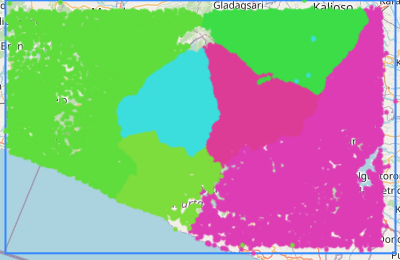
\includegraphics[]{figures/partition_level_4.png}
    \caption{Partisi hasil algoritma Inertial Flow dengan ukuran minimum partisi $U=2^{17}$ untuk graf jaringan jalan peta Openstreetmap wilayah Surakarta, Daerah Istimewa Yogyakarta, dan Klaten. Graf memiliki jumlah simpul sebanyak 481.978 dan jumlah sisi sebanyak 1.222.793.}
    \label{fig:inertial-flow}
\end{figure}
